% https://es.overleaf.com/latex/templates/project-report/jpzczmpsdzwm

%%% Preamble
\documentclass[paper=leter, fontsize=11pt]{scrartcl}
\usepackage[utf8]{inputenc}
\usepackage[spanish,mexico]{babel}
\usepackage[T1]{fontenc}    % use 8-bit T1 fonts
\usepackage{lmodern}
\usepackage{hyperref}       % hyperlinks
\usepackage{lipsum}
\usepackage[square,numbers]{natbib}

\usepackage[protrusion=true,expansion=true]{microtype}	
\usepackage{amsmath,amsfonts,amsthm} % Math packages
\usepackage[pdftex]{graphicx}
\usepackage{url}
 
\usepackage{booktabs}
\usepackage[table,xcdraw]{xcolor}

\usepackage{tikz}
\usetikzlibrary{positioning,matrix, arrows.meta}

\usepackage{caption} 
\usepackage{subcaption}


\usepackage{listings}
\lstdefinestyle{mystyle}{ 
    basicstyle=\ttfamily\footnotesize,
    breakatwhitespace=false,         
    breaklines=true,                 
    captionpos=b,                    
    keepspaces=true,                 
    numbers=left,                    
    numbersep=5pt,                  
    showspaces=false,                
    showstringspaces=false,
    showtabs=false,                  
    tabsize=4
}

\lstset{style=mystyle}
\renewcommand{\lstlistingname}{Código}


\selectlanguage{spanish}
\usepackage[spanish,onelanguage,ruled]{algorithm2e}


%%% Custom sectioning
\usepackage{sectsty}
\allsectionsfont{\centering \normalfont\scshape}


%%% Custom headers/footers (fancyhdr package)
\usepackage{fancyhdr}
\pagestyle{fancyplain}
\fancyhead{}											% No page header
\fancyfoot[L]{}											% Empty 
\fancyfoot[C]{}											% Empty
\fancyfoot[R]{\thepage}									% Pagenumbering
\renewcommand{\headrulewidth}{0pt}			% Remove header underlines
\renewcommand{\footrulewidth}{0pt}				% Remove footer underlines
\setlength{\headheight}{13.6pt}


%%% Equation and float numbering
\numberwithin{equation}{section}		% Equationnumbering: section.eq#
\numberwithin{figure}{section}			% Figurenumbering: section.fig#
\numberwithin{table}{section}				% Tablenumbering: section.tab#


%%% Maketitle metadata
\newcommand{\horrule}[1]{\rule{\linewidth}{#1}} 	% Horizontal rule

%%% https://tex.stackexchange.com/a/118217
\usepackage{mathtools}
\DeclarePairedDelimiter\ceil{\lceil}{\rceil}
\DeclarePairedDelimiter\floor{\lfloor}{\rfloor}

\usepackage{amsmath}

\usepackage{tikz}

\title{
		%\vspace{-1in} 	
		\usefont{OT1}{bch}{b}{n}
		\normalfont \normalsize \textsc{Posgrado de Ingeniería de Sistemas} \\ [25pt]
		\horrule{0.5pt} \\[0.4cm]
		\huge Distribución de Poisson \\
		\horrule{2pt} \\[0.5cm]
}
\author{
		\normalfont 								\normalsize
        Alberto Benavides\\[-3pt]		\normalsize
        \today
}
\date{}


%%% Begin document
\begin{document}
\maketitle

\section{Introducción}

La distribución de Poisson modela la probabilidad de que un evento con media $\lambda$ se repita $k$ dada la función
\begin{equation}
    P(X = k) = \frac{\lambda ^ k \times e ^ {- \lambda}}{k!}.
\end{equation}

En el presente reporte se explorarán maneras de generar esta función de distribución a partir de experimentos computacionales realizados en el lenguaje \texttt{R} \cite{r} ejecutadas en un cuaderno de \texttt{Jupyter} \cite{jupyter}.

\section{Visualización de la distribución de Poisson}

Se puede utilizar la función \texttt{rpois(n, L)} para generar \texttt{n} valores aleatorios obtenidos de una distribución de Poisson con $\lambda$ igual a \texttt{L}. Un ejemplo de $1000$ números generados aleatoriamente de esta manera puede revisarse en la figura \ref{poisson} (p. \pageref{poisson}) en forma de histograma.

\begin{figure}
    \centering
    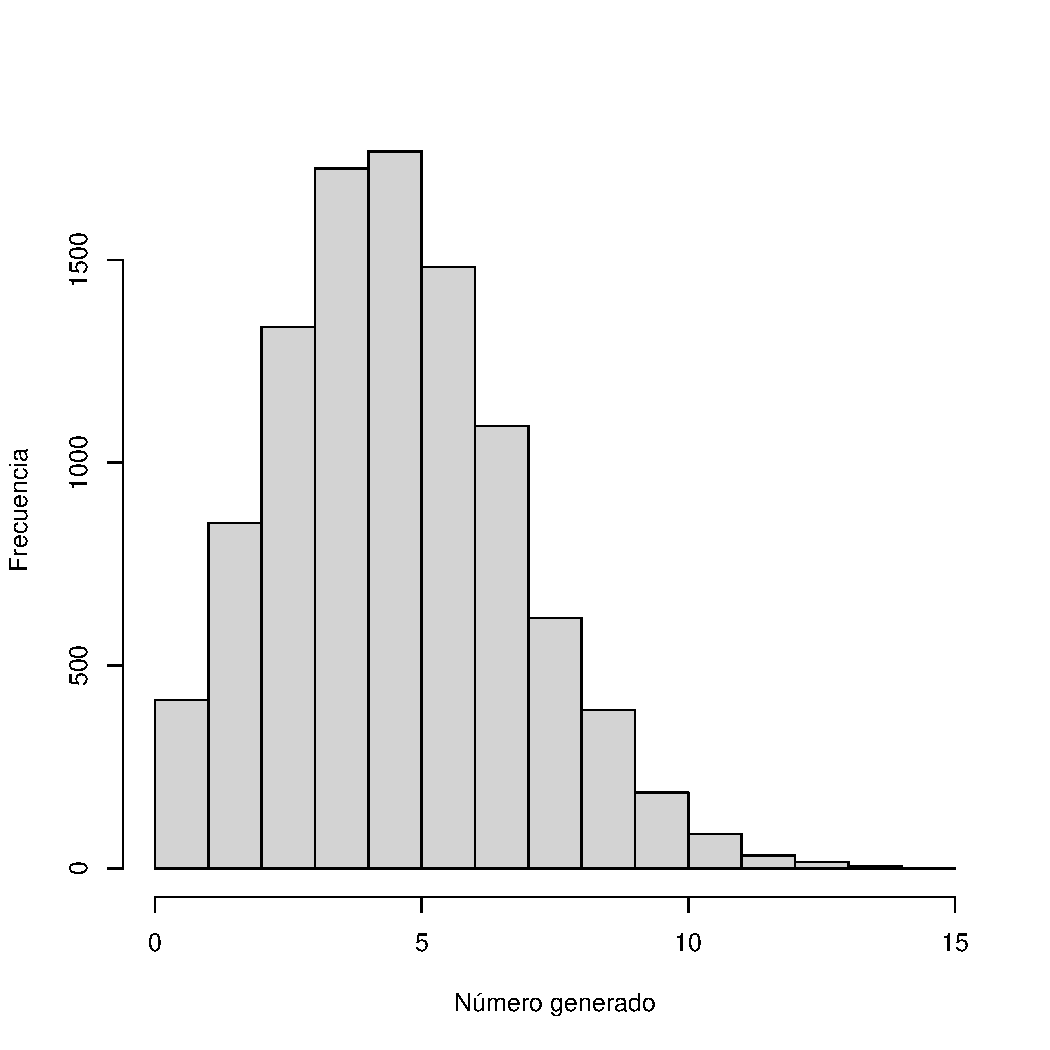
\includegraphics[width=1\textwidth]{poisson.pdf}
    \caption{Histograma de $1000$ valores aleatorios generados por una distribución de Poisson con $\lambda = 5$.}
    \label{poisson}
\end{figure}

\section{Generación a partir de experimentos computacionales}

Dada la definición de la distribución de Poisson como la probabilidad de que sucedan $k$ eventos con media $\lambda$, se pueden realizar experimentos computacionales que generen histogramas de distribución similares a los de Poisson a partir de funciones que generen números pseudoaleatorios obtenidos de distribuciones normales, uniformes y exponenciales. Una manera que se idea para lograrlo consiste en un ciclo que se repita $n = 10000$ veces en el que se sumen $m = 100$ números generados aleatoriamente a partir de una distribución normal con media $\mu = 5$ y desviación estándar $\sigma = 1$. Este procedimiento se refleja en el algoritmo mostrado en \ref{norm_alg} y las $n$ sumas generadas se despliegan en el histograma de la figura \ref{norm} (p. \pageref{norm}) junto al histograma obtenido por la función \texttt{rpois(n, m * mu)}. Es importante resaltar en este procedimiento que como ya se conoce de antemano $\mu$ y también la cantidad de veces $m$ que se suman números pseudoaleatorios obtenidos de una distribución normal, se puede calcular la media de la distribución generada por la multiplicación de ambos valores, de modo que se puede utilizar en la distribución de Poisson $\lambda = m \times \mu$.

\begin{algorithm}
	\caption{Algoritmo para generar una distribución de Poisson a partir de sumas de números aleatorios generados a partir de una distribución normal.}
	\label{norm_alg}
	\SetAlgoLined

    \(n = 10000\)\;
    \(m = 100\)\;
    \(\mu = 5\)\;
    \(\sigma = 1\)\;
    \(\texttt{resultados} = [] \)\;
	\For{\(i \in n\)}{
        \( \text{Agregar a \texttt{resultados}} \sum{\mathcal{N}(\mu, \sigma)} \)\;
	}
\end{algorithm}

\begin{figure}
    \begin{subfigure}{.5\textwidth}
        \centering
        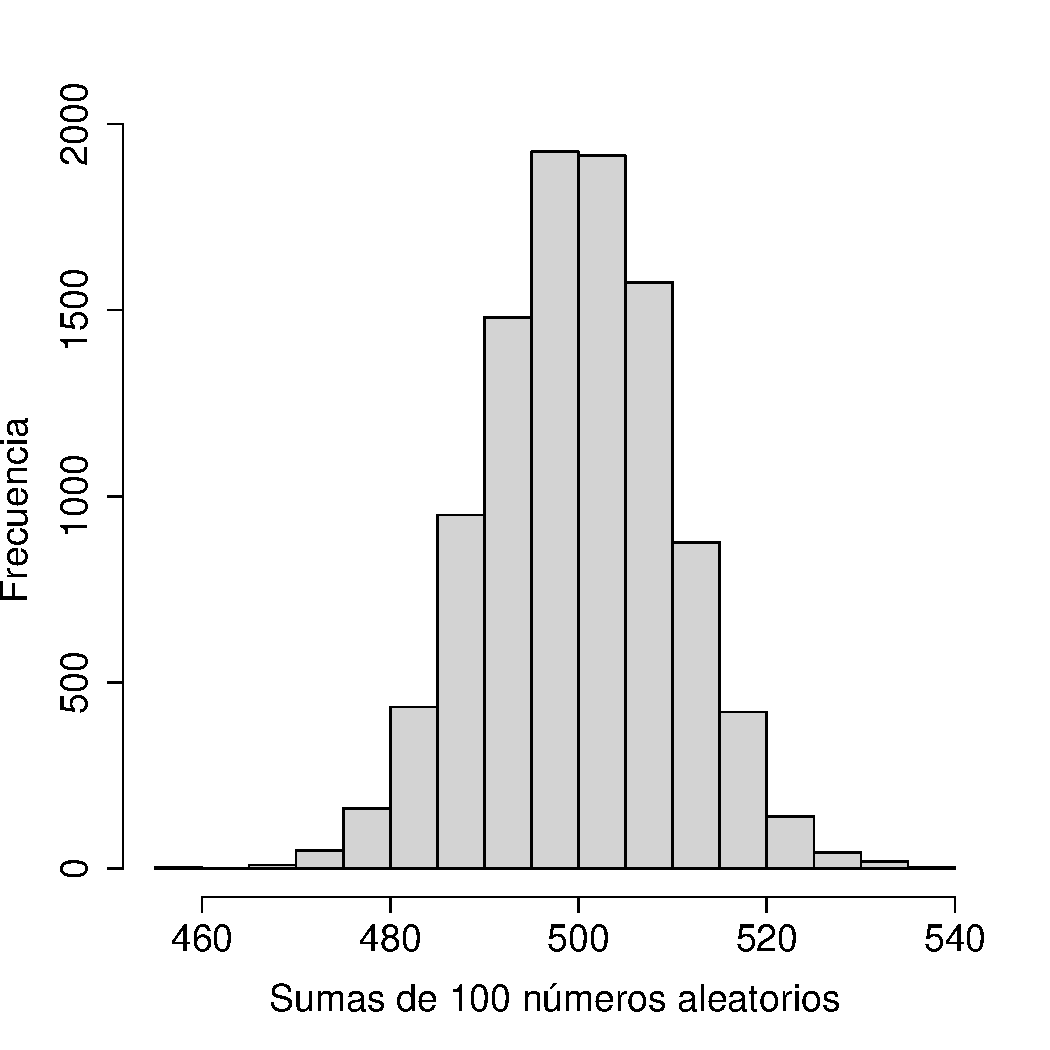
\includegraphics[scale=0.4]{norm.pdf}
        \caption{Generador a partir de distribución normal.}
        \label{norm_izq}
    \end{subfigure}
    \begin{subfigure}{0.5\textwidth}
        \centering
        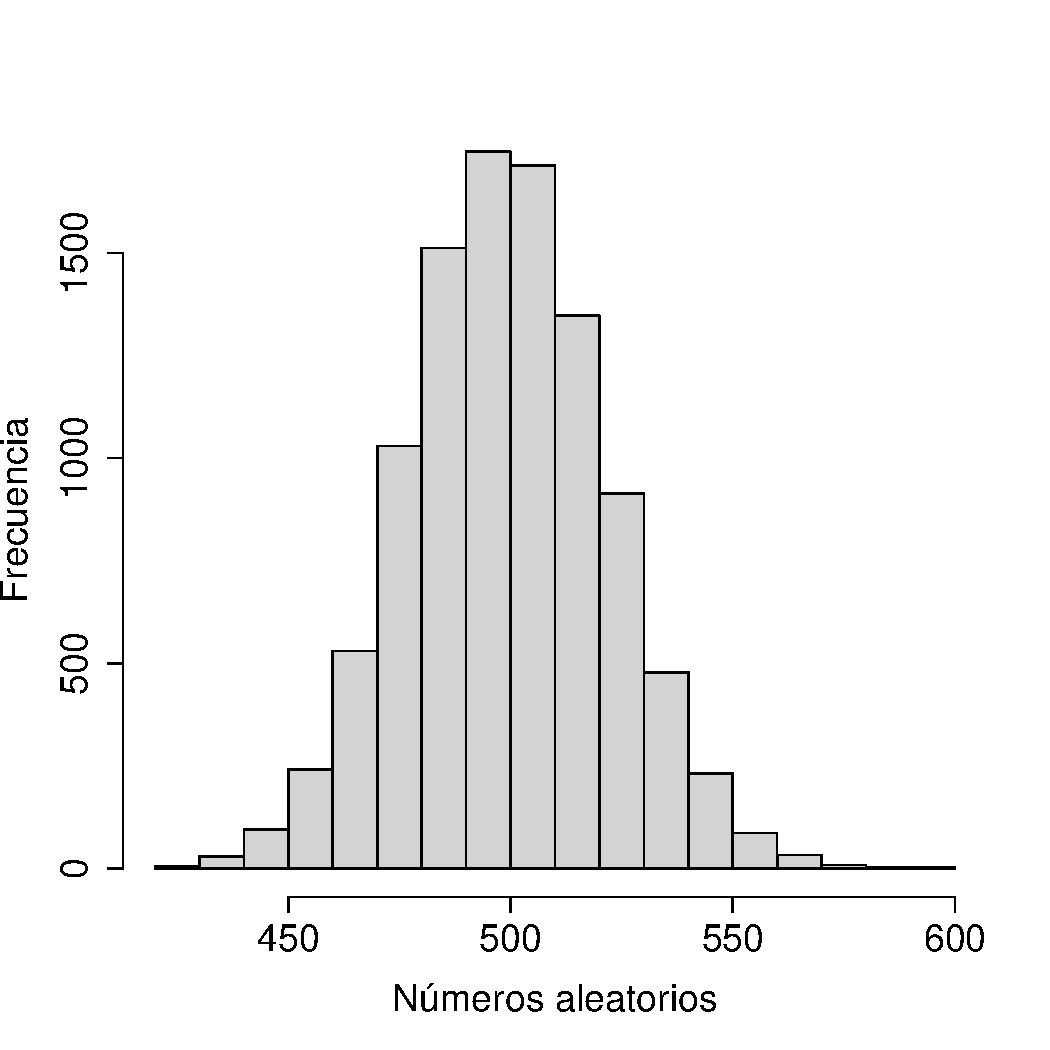
\includegraphics[scale=0.4]{norm_poisson.pdf}
        \caption{Valores generados por distribución $\text{Poisson}(\lambda)$}
        \label{norm_der}
    \end{subfigure}
    \caption{Histograma de $10000$ valores generados por la suma de $100$ números aleatorios con una distribución $\mathcal{N}(5, 1)$ \ref{norm_izq} y el obtenido por la función \texttt{rpois} de \texttt{R} \ref{norm_der}.}
    \label{norm}
\end{figure}

Este mismo procedimiento se puede utilizar con números generados a partir de una distribución uniforme $\mathcal{U}(0, 1)$. La diferencia en este caso es que la media de la suma de los valores debe dividirse entre dos debido a que una distribución uniforme tiene una $E(X) = 0.5$. Los histogramas de este generador y distribución de Poisson se hallan en las figuras \ref{unif_izq} y \ref{unif_der} (p. \pageref{unif}). De manera análoga, se puede utilizar una distribución binomial $\mathcal{B}(m, p)$ en la que la multiplicación de $n \times m \times p$ da por resultado la media de la distribución generada y, por lo mismo, el parámetro $\lambda$ que usa la distribución de Poisson. Los histogramas de estas funciones pueden verse en \ref{binom_izq} y \ref{binom_der} (p. \pageref{unif}).

\begin{figure}
    \begin{subfigure}{.5\textwidth}
        \centering
        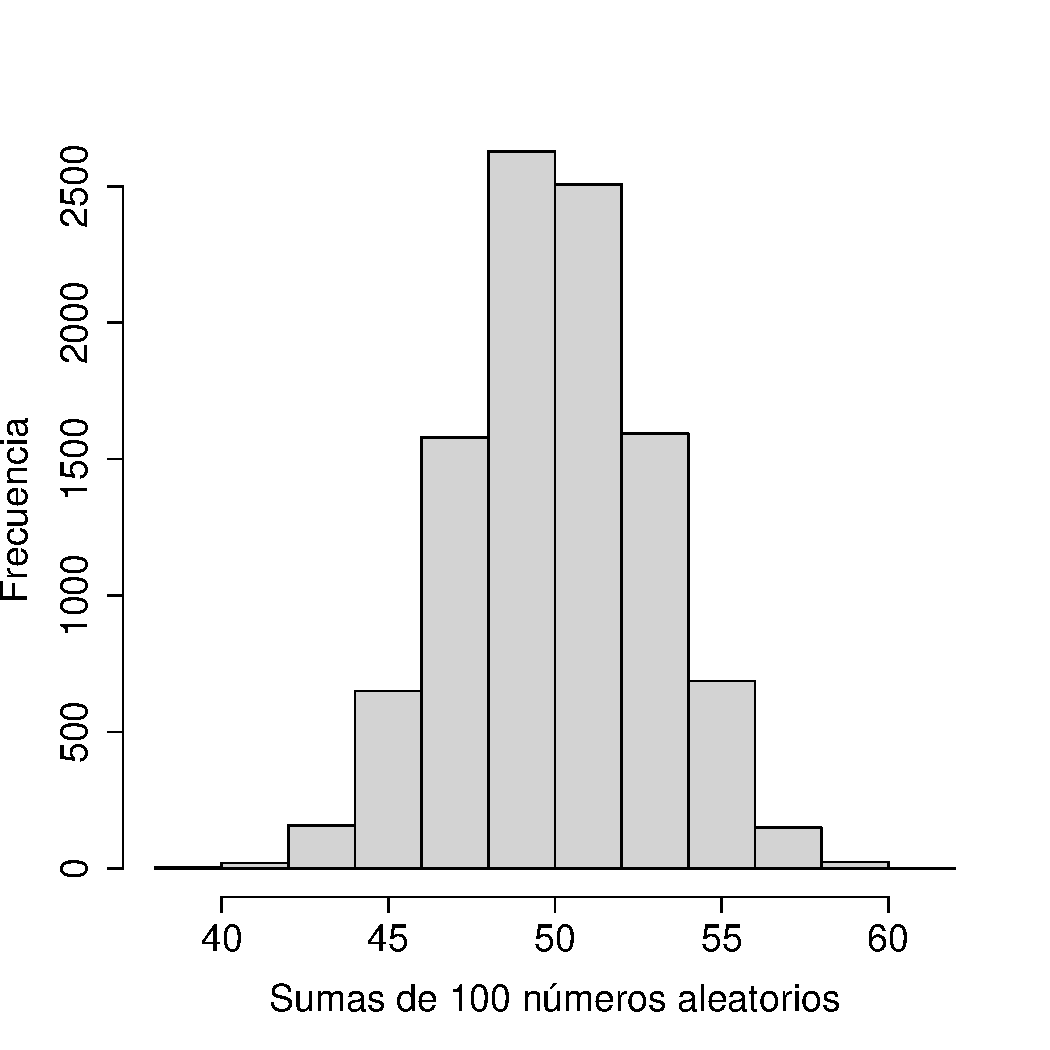
\includegraphics[scale=0.4]{unif.pdf}
        \caption{Generador a partir de distribución uniforme.}
        \label{unif_izq}
    \end{subfigure}
    \begin{subfigure}{0.5\textwidth}
        \centering
        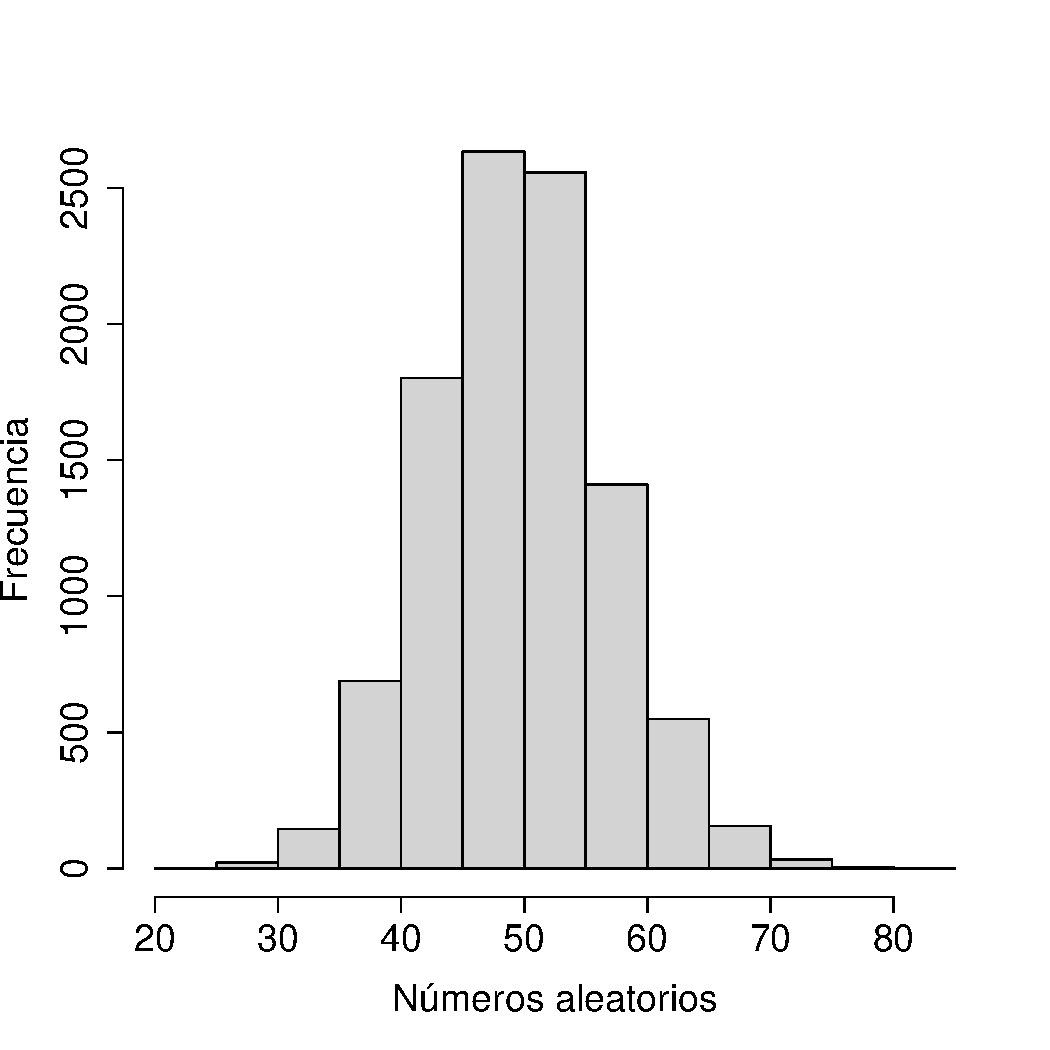
\includegraphics[scale=0.4]{unif_poisson.pdf}
        \caption{Valores generados por distribución $\text{Poisson}(\lambda)$}
        \label{unif_der}
    \end{subfigure}

    \begin{subfigure}{.5\textwidth}
        \centering
        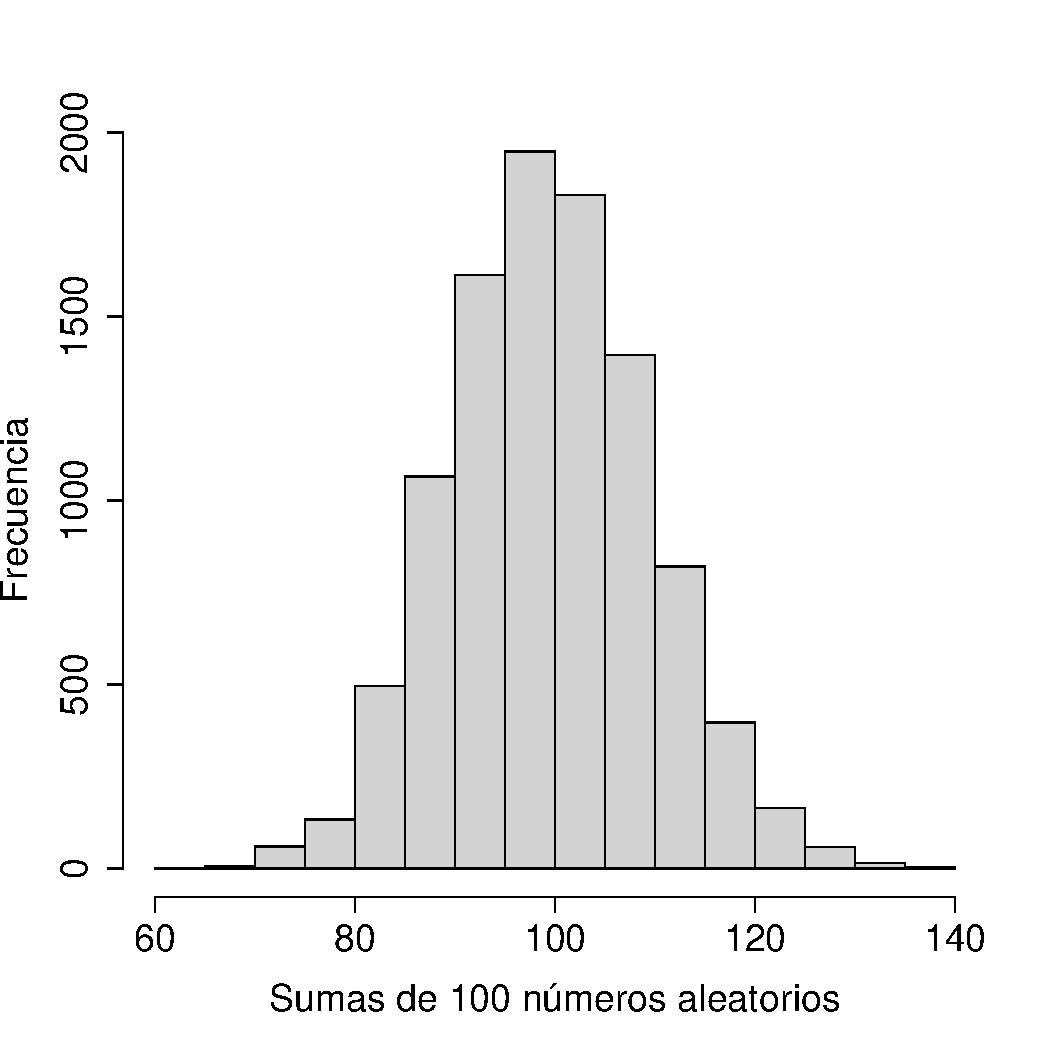
\includegraphics[scale=0.4]{binom.pdf}
        \caption{Generador a partir de distribución binomial.}
        \label{binom_izq}
    \end{subfigure}
    \begin{subfigure}{0.5\textwidth}
        \centering
        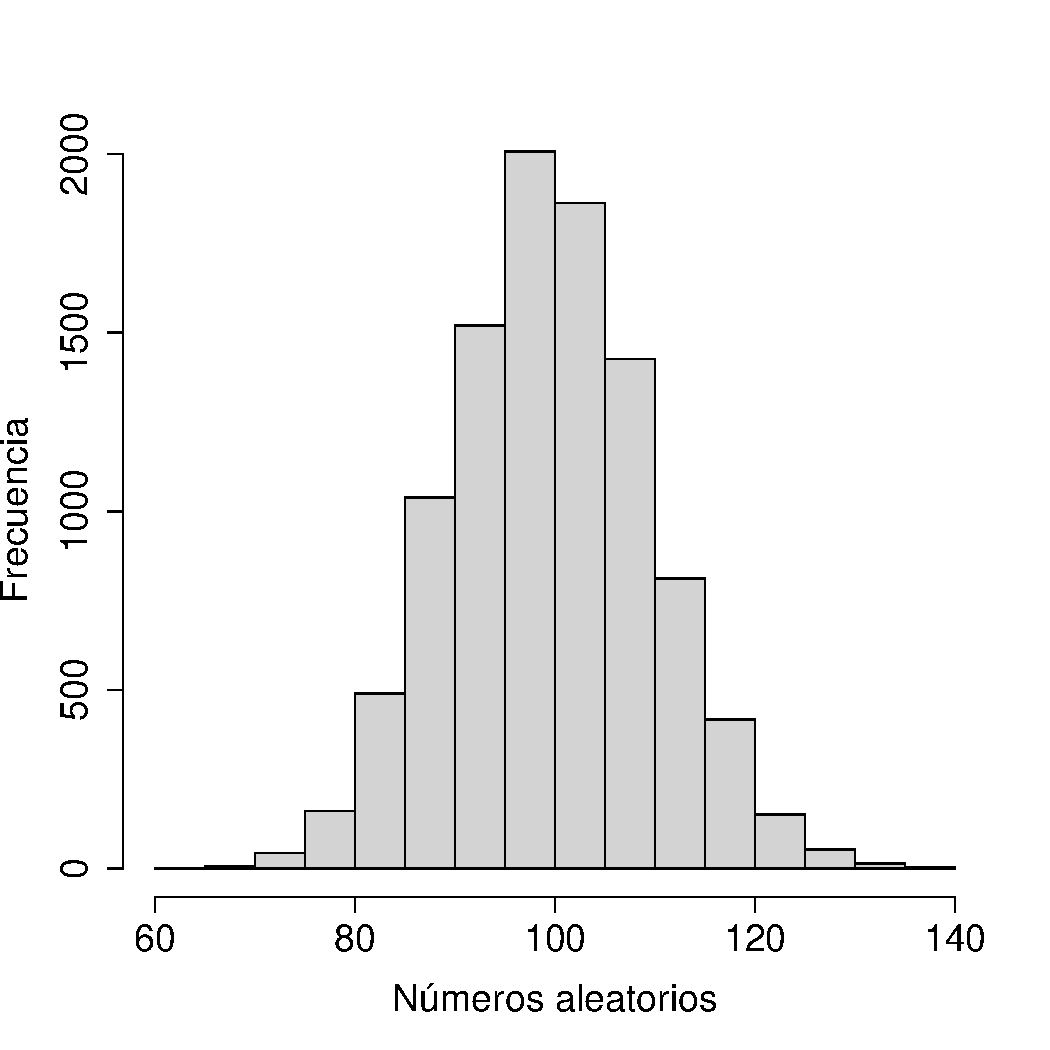
\includegraphics[scale=0.4]{binom_poisson.pdf}
        \caption{Valores generados por distribución $\text{Poisson}(\lambda)$}
        \label{binom_der}
    \end{subfigure}
    \caption{Histograma de $10000$ valores generados por la suma de $100$ números aleatorios con una distribución $\mathcal{U}(0, 1)$ \ref{unif_izq}, una binomial $\mathcal{B}(100, 0.01)$ \ref{binom_izq} y los obtenido por la función \texttt{rpois} de \texttt{R}  para cada una respectivamente, \ref{unif_der} y \ref{binom_der}.}
    \label{unif}
\end{figure}

\section{Comparación entre distribuciones}

Los histogramas de distribuciones parecen semejantes, sin embargo una manera rápida de comprobar si las distribuciones son iguales consiste en usar diagramas de cajas y bigotes. En la figura \ref{boxplots} (p. \pageref{boxplots}) se puede constatar que la distribución uniforme es la que presenta una distribución distinta a las demás.

\begin{figure}
    \centering
    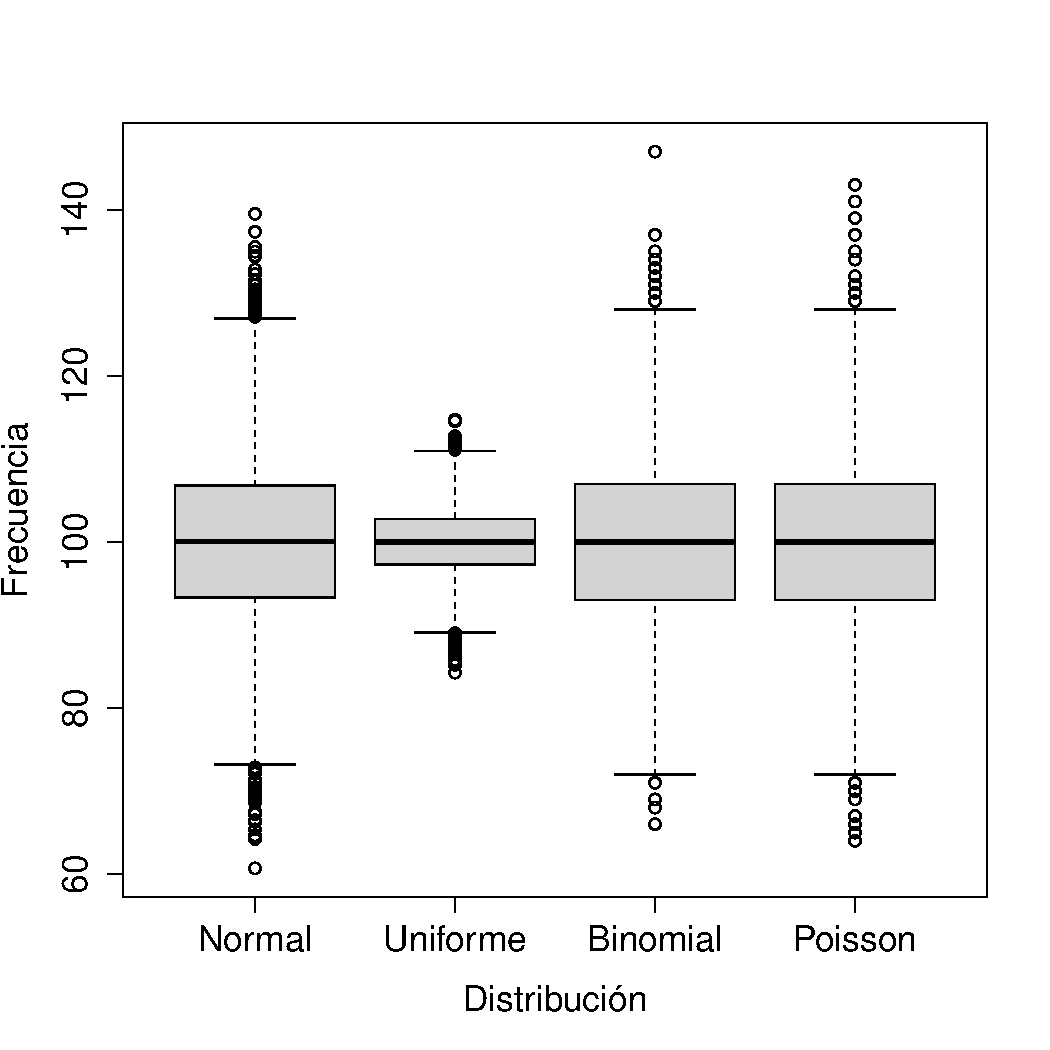
\includegraphics[width=1\textwidth]{boxplots.pdf}
    \caption{Diagramas de cajas y bigotes generados por la función detallada en \ref{norm_alg} para las distribuciones normal, uniforme y binomial, mientras la distribución de Poisson utiliza la función \texttt{rpois} de \texttt{R}.}
    \label{boxplots}
\end{figure}

\bibliographystyle{plainnat}
\bibliography{Biblio}

\end{document}